\section{Cours 3}
\subsection{Dualité dans la programmation linéaire}
maximiser 2x$_1$+3x$_2$ avec:
\begin{itemize}
	\item 4x$_1$+8x$_2\leq$12
	\item 2x$_1$+x$_2\leq$3
	\item 3x$_1$+2x$_2\leq$4
	\item x$_1$,x$_2\geq$0
\end{itemize}
L'objectif est de calculer les bornes supérieures pour l'optimum sans résoudre le programme linéaire.
\begin{enumerate}
	\item Notons que 2x$_1$+3x$_2\leq$4x$_1$+8x$_2\leq$12$\Rightarrow$OPT$\leq$12
	\item Notons aussi 2x$_1$+3x$_2\leq\frac{1}{2}$(4x$_1$+8x$_2$)$\leq$6$\Rightarrow$OPT$\leq$6
	\item Aussi 2x$_1$+3x$_2$=$\frac{1}{3}$(4x$_1$+8x$_2$)+$\frac{1}{3}$(2x$_1$+x$_2$)$\leq\frac{12}{3}$+
	$\frac{3}{3}$=5$\Rightarrow$OPT$\leq$5
\end{enumerate}
On note (D), le programme linéaire dual du programme linéaire.
\newpage
\textbf{Cas général:}
\begin{figure}[h!]
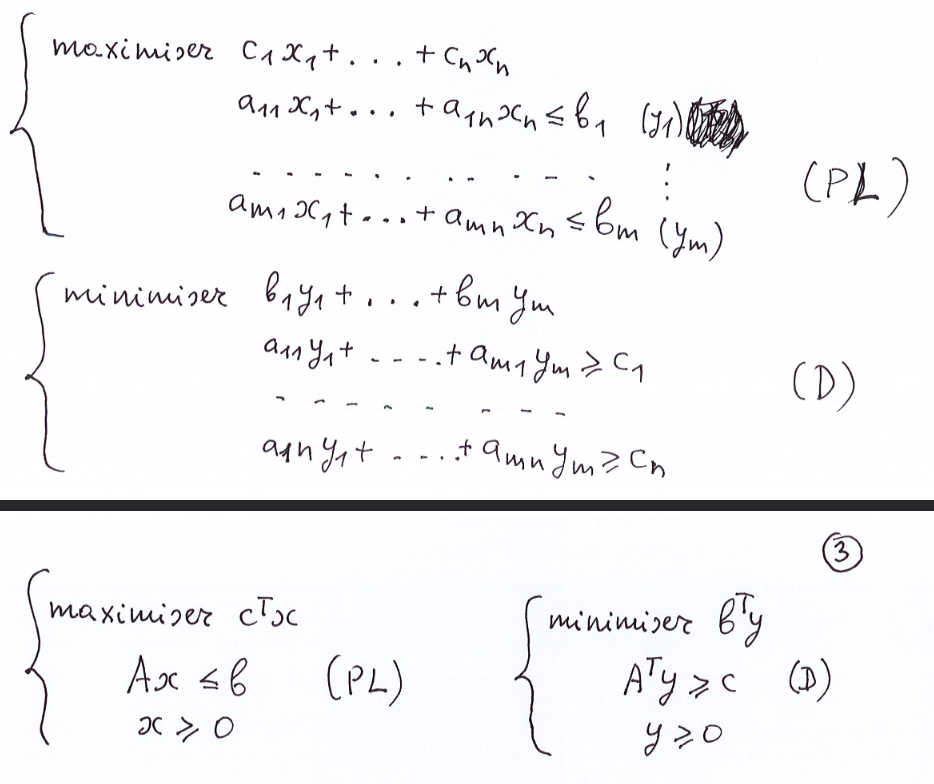
\includegraphics[width=\linewidth,height=0.75\textheight]{notes/algorithme/cas_general_dualite.png}
\end{figure}

\textbf{Proposition:\\}
Si x est une solution admissible du programme linéaire, et y est une solution admissible du dual, alors
c$^t$x $\leq$b$^t$y.

\textbf{Théorème:\\}
Si x$^*$=(x$_1^*$, ..., x$_n^*$) est une solution optimale du programme linéaire, alors le dual admet une
solution optimale y$^*$=(y$_1^*$, ..., y$_m^*$), et $\Sigma_{j=1}^n~c_j~x_j^*$ =  $\Sigma_{i=1}^m~b_i~y_i^*$.\\
Donc, le programme linéaire et le dual on la même valeur de l'optimum.

\textbf{Proposition:\\}
Soit z =z$_0+\Sigma_{i=1}^{n+m}~d_ix_i$, l'expression de la fonction objectif dans le dernier dictionnaire des
programmes linéaires, avec
\begin{itemize}
	\item d$_i$=0 si i$\in$B
	\item d$_i\leq$0 si i$\in$N
\end{itemize}
Alors, y$_1^*$=-d$_{n+1}$, ..., y$_m^*$=-d$_{n+m}$ est une solution optimale du dual.

\textbf{Conculsion:\\}
Pour résoudre le programme linéaire et son dual à la fois, il faut résoudre soit l'un, soit l'autre. Le plus simple,
de préférence.

\subsection{Théorème des écarts complémentaire}
\textbf{Théorème:\\}
une solution admissible x$_1^*$, ..., x$_n^*$ du primal est optimale si et seulement si il existe des nombres
y$_1^*$, ..., y$_m^*$ tels que:
\begin{itemize}
	\item si $\Sigma_{j=1}^n~a_{ij}x_j^*<b_i$, alors y$_i^*$=0
	\item si x$_j^*>$0, alors $\Sigma~a_{ij}y_i^*$=c$_j$
\end{itemize}
et tels que;
\begin{itemize}
	\item $\Sigma~a_{ij}y_i^* \geq c_j$, j = 1, ..., n
	\item j$_i^*\geq$0, i = 1, ..., m
\end{itemize}
Dans ce cas, y$^*$=(y$_1^*$, ..., y$_m^*$) est une solution optimale du dual.

\begin{figure}[!ht]
\subsection{La signification économique du dual}
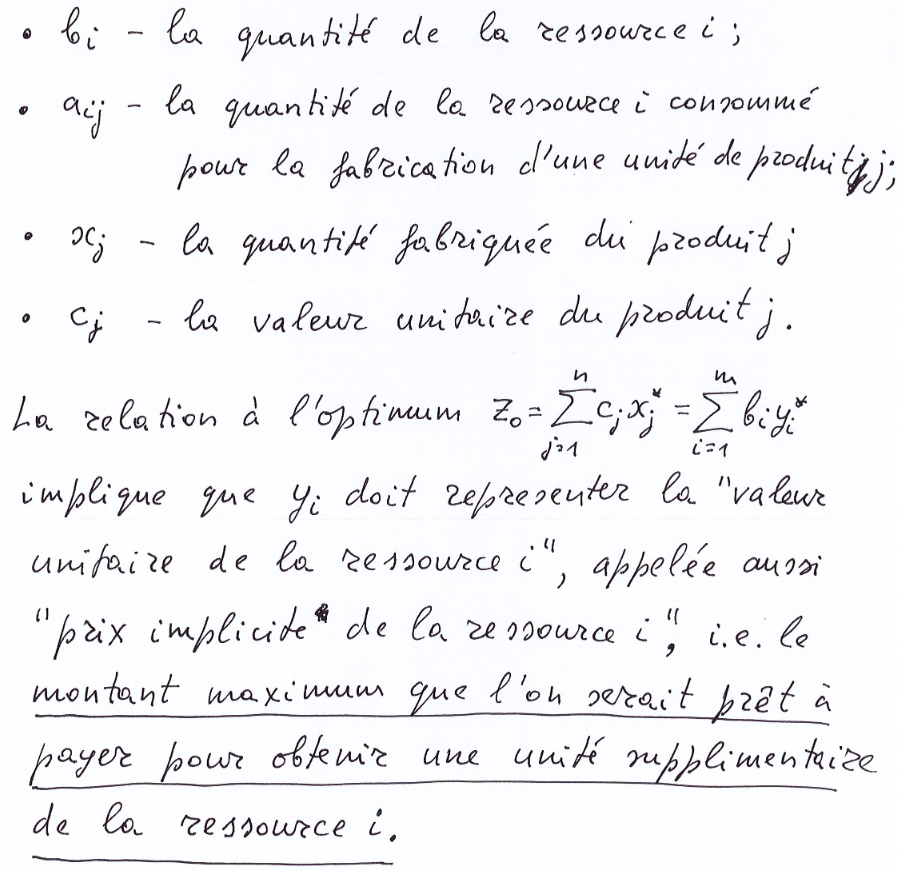
\includegraphics[width=\linewidth,height=0.75\textheight]{notes/algorithme/sig_eco_dualite.png}
\end{figure}

\begin{figure}[!ht]
\subsection{Problème dual-réalisable}
Un programme linéaire est dual-réalisable si les coefficients c$_j$ de la fonction objectif sont tous négatifs.
Dans ce cas, à la place de la méthode à deux phases, on peux utiliser le dual.
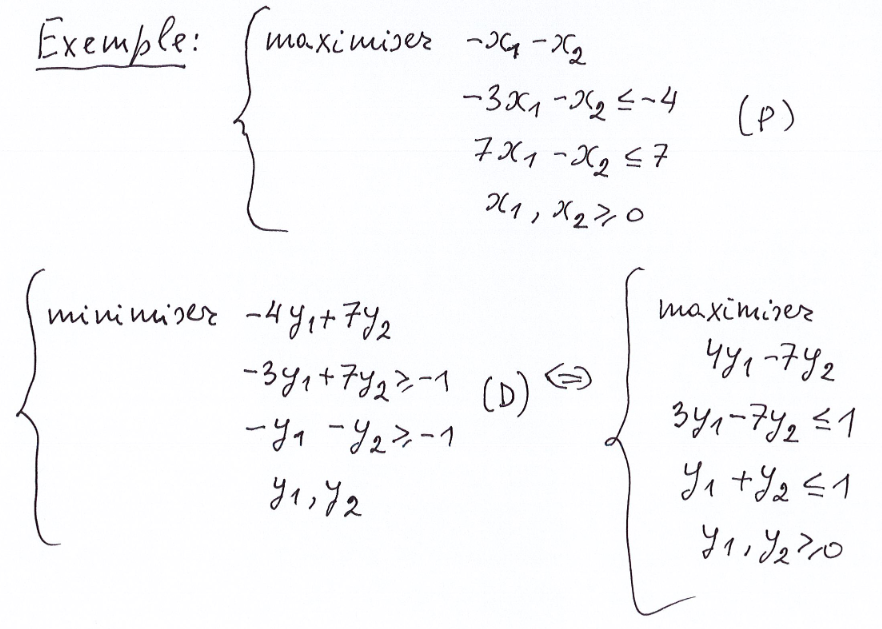
\includegraphics[width=\linewidth,height=0.75\textheight]{notes/algorithme/ex_pb_dual_rea.png}
\end{figure}
